\documentclass[11pt]{article}
\usepackage{amssymb}
\usepackage{tipa}
\usepackage{amsmath}
\usepackage[scr]{rsfso}
\usepackage{graphicx}
\usepackage{float}

\newcommand{\then}{\rightarrow} 
\newcommand{\bicond}{\leftrightarrow}
\newcommand{\powerset}[1]{\mathscr{P}(#1)}
\newcommand{\family}[1]{\mathcal{#1}}
\newcommand{\dprime}{{\prime \prime}}

\title{\textbf{How to Prove It} \\ {\Large\itshape Daniel J. Velleman} \\ {\Large\itshape Chapter 4.4: Ordering Relations}}

\author{\textbf{Nathaniel Curnick} \\ \textit{Textbook Solutions}}

\date{}

%----------------------------------------------------------------------------------------

\begin{document}

\maketitle

\section*{Exercise 1}

In each case, say whether or not $R$ is a partial order on $A$. If so, is it a 
total order?

\noindent (a) $A = \{a, b, c\}$, $R = \{(a,a),(b,a),(b,b),(b,c),(c,c)\}$

Partial order, but not a total order since $(a,c) \notin R$ and $(c, a) \notin R$

\noindent (b) $A = \mathbb{R}$, $R = \{(x, y) \in \mathbb{R} \times \mathbb{R} | |x| \leq |y|\}$

Not partial order since $(-1, 1) \in R$ and $(1, -1) \in R$ but $-1 \neq 1$.

\noindent (c) $A = \mathbb{R}$, $R = \{(x, y) \in \mathbb{R} \times \mathbb{R} | |x| < |y| \text{ or } x = y\}$

Partial order

\section*{Exercise 2}

In each case, say whether or not $R$ is a partial order on $A$. If so, is it a 
total order?

\noindent (a) $A = \text{ the set of all words of English}$,
$R = \{(x, y) \in A \times A | \text{ the word } y \text{ occurs at least as late in the alphabetical order as the word } x\}$

Total order (you can order all words alphabetically)

\noindent (b) $A = \text{ the set of all words of English}$,
$R = \{(x, y) \in A \times A | \text{ the first letter of the word } y \text{ occurs at least as late in the alphabetical order as the first letter of the word } x\}$

Not a partial order as e.g. $(\text{car, cab}) \in R$ and $(\text{cab, car}) \in R$
but $\text{car} \neq \text{cab}$

\noindent (c) $A = \text{ the set of all countries in the world }$, 
$R = \{(x, y) \in A \times A | \text{ the population of country } y \text{ is at least as large as the population of the country } x\}$

A partial order, as you can mostly order the countries by population except for 
the cases where countries have the exact same number of people 

\section*{Exercise 3}

In each case find all minimal and maximal elements of $B$. Also find, if they 
exist, the largest and mallest elements of $B$, and the least upper bound and
greatest lower bound of $B$.

\noindent (a) $R = \text{ the relation shown in the below graph}$, $B = \{2,3,4\}$

\begin{figure}[H]
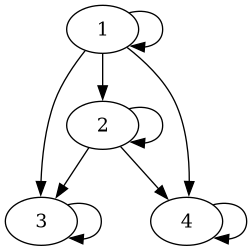
\includegraphics[height=0.25\textheight]{4_4_images/4_4_3a.png}
\end{figure}


\begin{itemize}
    \item Maximal elements: 3, 4
    \item Miniaml element: 1
    \item Largest element: N/A 
    \item Smallest element: 1
    \item Least upper bound: N/A 
    \item Greatest lower bound: 1
\end{itemize}

\noindent (b) $R = \{(x,y) \in \mathbb{R} \times \mathbb{R} | x \leq y\}$,
$B = \{x \in \mathbb{R} | 1 \leq x < 2\}$

\begin{itemize}
    \item Maximal elements: N/A
    \item Miniaml element: 1
    \item Largest element: N/A 
    \item Smallest element: 1
    \item Least upper bound: 2
    \item Greatest lower bound: 1
\end{itemize}

\noindent (c) $R = \{(x,y) \in \powerset{\mathbb{N}} \times \powerset{\mathbb{N}} | x \subseteq y\}$,
$B = \{x \in \powerset{\mathbb{N}} | x \text{ has at most 5 elements} \}$

\begin{itemize}
    \item Maximal elements: Every 5 element set
    \item Miniaml element: $\emptyset$
    \item Largest element: N/A 
    \item Smallest element: $\emptyset$
    \item Least upper bound: N/A
    \item Greatest lower bound: $\emptyset$
\end{itemize}

\section*{Exercise 4}

Suppose $R$ is a relation on $A$. You might think that $R$ could not be both 
antisymmetric and symmetric, but this isn't true. Prove that $R$ is both 
antisymmetric and symmetric iff $R \subseteq i_A$.

Suppose that $R$ is both antisymmetric and symmetric. Suppose that 
$(x, y) \in R$. Since $R$ is symmetric $(y, x) \in R$ and since 
$R$ is antisymmetric it follows that $x = y$. Therefore, $(x, y) \in i_A$.
Since $(x, y)$ was arbitrary, this shows that $R \subseteq i_A$.

Suppose now that $R \subseteq i_A$. Suppose $(x, y) \in R$. Then
$(x, y) \in i_A$, so $x=y$ and therefore $(y, x) = (x, y) \in R$.
This shows that $R$ is symmetric. To show that $R$ is antisymmetric suppose that 
$(x, y) \in R$ and $(y, x) \in R$, then $(x, y) \in i_A$, so $x = y$.

\section*{Exercise 5}

Suppose $R$ is a partial order on $A$ and $B \subseteq A$. Prove that 
$R \cap (B \times B)$ is a partial order on $B$.

Suppose $x \in B$. Since $B \subseteq A$, then $x \in A$. Since $R$ is reflexive
on $A$, then $(x, x) \in R$. As $(x, x) \in B \times B$ so 
$(x, x) \in R \cap (B \times B)$. Since $x$ was an arbitrary element, this 
shows that $R \cap (B \times B)$ is reflexive on $B$.

Suppose $(x, y) \in R \cap (B \times B)$ and $(y, z) \in R \cap (B \times B)$.
Then $(x, y) \in R$ and $(y, z) \in R$, so since $R$ is transitive then
$(x, z) \in R$. Also, $(x, y) \in B \times B$ and $(y, z) \in B \times B$, so 
$x \in B$ and $z \in B$ and so $(x, z) \in B \times B$. Thus, 
$(x, z) \in R \cap (B \times B)$ so $R \cap (B \times B)$ is transitive.

Finally, suppose $(x, y) \in R \cap (B \times B)$ and $(y, x) \in R \cap (B \times B)$.
Then $(x, y) \in R$ and $(y, x) \in R$. Since $R$ is antisymmetric $x = y$.
Therefore $R \cap (B \times B)$ is antisymmetric.

Since $R \cap (B \times B)$ is reflexive, transitive and antisymmetric it is a 
partial order on $B$.

\section*{Exercise 6}

Suppose $R_1$ and $R_2$ are partial orders on $A$. For each part, give either a 
proof or a counterexample to justify your answer. 

\noindent (a) Must $R_1 \cap R_2$ be a partial order on $A$?

Since $R_1$ and $R_2$ are both reflexive, then $(x, x) \in R_1$ and $(x, x) \in R_2$ 
so $(x, x) \in R_1 \cap R_2$ so it is reflexive.

Suppose $(x, y) \in R_1 \cap R_2$ and $(y, z) \in R_1 \cap R_2$. Then 
$(x, y) \in R_1$ and $(y, z) \in R_1$, since $R_1$ is transitive then 
$(x,z) \in R_1$. By symmetry $(x,z) \in R_2$. Therefore $(x, z) \in R \cap R_2$,
so it is transitive.

Suppose $(x, y) \in R_1 \cap R_2$ and $(y, x) \in R_1 \cap R_2$. Then 
$(x, y) \in R_1$ and $(y, x) \in R_1$. But, since $R_1$ is antisymmetric
$x=y$. By symmetry, $y=x$ for $R_2$ also. Thus $R_1 \cap R_2$ is antisymmetric.

Since $R_1 \cap R_2$ is reflexive, transitive and antisymmetric it must be a 
partial order.

\noindent (b) Must $R_1 \cup R_2$ be a partial order on $A$?

No. Consider if $(x, y) \in R_1$ and $(y, x) \in R_2$ then $(x, y)$ and 
$(y, x)$ would be elements of $R_1 \cup R_2$ which would mean it is not 
antisymmetric and so it is not a partial order.

\section*{Exercise 7}

Suppose $R_1$ is a partial order on $A_1$, $R_2$ is a partial order on $A_2$ 
and $A_1 \cap A_2 \neq \emptyset$

\noindent (a) Prove that $R_1 \cup R_2$ is a partial order on $A_1 \cup A_2$

Since $R_1$ is a partial order on $A_1$, then it is reflexive. Thus, 
$(x_1, x_1) \in R_1$ whyere $x_1 \in A_1$. By symmetry, $(x_2, x_2) \in R_2$
where $x_2 \in A_2$. Thus, $(x_1, x_1) \in R_1 \cup R_2$ and 
$(x_2, x_2) \in R_1 \cup R_2$ and $x_1 \in A_1 \cup A_2$ and 
$x_2 \in A_1 \cup A_2$. Thus, $R_1 \cup R_2$ is reflexive on $A_1 \cup A_2$.

Suppose $x,y,z$ are elements of $A_1$. Since $A_1 \cap A_2 = \emptyset$, then
$x,y,z$ are not elements of $A_2$. Since $R_1$ is reflexive, then 
$(x,y) \in R_1$, $(y,z) \in R_1$ and $(x,z) \in R_1$. 
Therefore, $x,y,z \in A_1 \cup A_2$ and $(x,y) \in R_1 \cup R_2$, 
$(y,z) \in R_1 \cup R_2$ and $(z,x) \in R_1 \cup R_2$. Since $A_1$ and $A_2$ have
no elements in common, the symmetrical argument holds for all transitive 
triplets in $A_1$. Thus, $R_1 \cup R_2$ is transitive on $A_1 \cup A_2$.

Since $R_1$ is antisymmetric, then $(x,y) \in R_1$ and $(y,x) \in R_1$ where
$x=y$. Since $A_1 \cup A_2 = \emptyset$ then no elements from $A_2$ can be 
introduced to make it so $(x,z) \in R_1 \cup R_2$ and $(z,x) \in R_1 \cup R_2$ 
where $z \neq x$. By symmetry, the same argument holds for $R_2$ and $A_1$. Thus,
$R_1 \cup R_2$ is antisymmetric. 

Thus, $R_1 \cup R_2$ is a partial order on $A_1 \cup A_2$.

\noindent (b) Prove that $R_1 \cup R_2 \cup (A_1 \times A_2)$ is a partial 
order on $A_1 \cup A_2$

We can use the same argument from part (a) to show it is reflexive 

We can also use the transitive argument from (a). Since $A_1 \cap A_2 = \emptyset$
then if $(x, y) \in A_1 \times A_2$ then $(y,z) \notin A_1 \times A_2$. Thus,
$A_1 \times A_2$ can not introduce any elements whose transitivity is questioned.

Again, the argument for antisymmetry holds from (a). Since $A_1 \cap A_2 = \emptyset$
then suppose $(x,y) \in A_1 \times A_2$, then $(x, y) \notin A_1 \cap A_2$.
Therefore, no elements which could break antisymmetry are introduced.

Thus, $R_1 \cup R_2 \cup (A_1 \times A_2)$ is a partial order on $A_1 \cup A_2$.

\noindent (c) Suppose that $R_1$ and $R_2$ are total orders. Are the partial 
orders in (a) and (b) also total orders?

First consider $R_1 \cup R_2$. If $a_1 \in A_1$ and $a_2 \in A_2$ then 
$(a_1, a_2) \notin R_1 \cup R_2$ and $(a_2, a_1) \notin R_1 \cup R_2$. 
Therefore, as long as $A_1 \neq \emptyset$ and $A_2 \neq \emptyset$ then 
$R_1 \cup R_2$ is not a total order.

Now consider $R_1 \cup R_2 \cup (A_1 \times A_2)$. 
Suppose $(x, y) \in A_1 \cup A_2$ There are four cases 

Case 1: $x \in A_1$ and $y \in A_1$. Then since $R_1$ is a total order on $A_1$
either $(x, y) \in R_1$ or $(y, x) \in R_1$, so either 
$(x, y) \in R_1 \cup R_2 \cup (A_1 \times A_2)$ or 
$(y,x) \in R_1 \cup R_2 \cup (A_1 \times A_2)$

Case 2: $x \in A_2$ and $y \in A_2$. Symmetrical to case 1.

Case 3: $x \in A_1$ and $y \in A_2$. Then, $(x, y) \in A_1 \times A_2$ so 
$(x, y) \in R_1 \cup R_2 \cup (A_1 \times A_2)$.

Case 4: $x \in A_2$ and $y \in A_1$. Symmetrical to case 3.

Therefore, $R_1 \cup R_2 \cup (A_1 \times A_2)$ is a total order

\section*{Exercise 8}

Suppose $R$ is a partial order on $A$ and $S$ is a partial order on $B$.
Define a relation $T$ on $A \times B$ as follows: 
$T = \{((a, b), (a^\prime, b^\prime)) \in (A \times B) \times (A \times B) | aRa^\prime \text{ and } bSb^\prime\}$
Show that $T$ is a partial order on $A \times B$. If both $R$ and $S$ are total 
orders, will $T$ also be a total order?

Suppose $(a, b) \in A \times B$. Since $R$ and $S$ are both reflexive, we have 
$aRa$ and $bSb$. By definition of $T$ it follows that $(a,b)T(a,b)$ therefore,
$T$ is reflexive.

Suppose that $(a,b)T(a^\prime, b^\prime)$ and 
$(a^\prime, b^\prime)T(a^\dprime, b^\dprime)$. 
Then $aRa^\prime$ and $a^\prime R a^\dprime$. Since $R$ is transitive then
$aRa^\dprime$. Similarly, $bSb^\prime$ and $b^\prime S b^\dprime$ so 
$bSb^\dprime$ therefore $(a, b)T(a^\dprime, b^\dprime)$.  Therefore, $T$ is 
transitive.

Suppose $(a, b) T (a^\prime, b^\prime)$ and $(a^\prime, b^\prime) T (a,b)$. 
Then $aRa^\prime$ and $a^\prime R a$ but since $R$ is antisymmetric then 
$a^\prime = a$. Similarly, $bSb^\prime$ and $b^\prime Sb$ but $S$ is antisymmetric
so $b = b^\prime$. Thus $(a,b) = (a^\prime,b^\prime)$. Thus, $T$ is antisymmetric.

Since $T$ is reflexive, transitive and antisymmetric it is therefore a partial order.

Even if $R$ and $S$ are both total orders, $T$ might not be a partial order.
For example, if $A = B = \mathbb{R}$ and 
$R = S = \{(x,y) \in \mathbb{R} \times \mathbb{R} | x \leq y \}$ then 
$((1,2), (2,1)) \notin T$ and $((2,1),(1,2)) \notin T$.

\section*{Exercise 9}

Suppose $R$ is a partial order on $A$ and $S$ is a partial order on $B$.
Define a relation $L$ on $A \times B$ as follows: 
$L = \{((a, b), (a^\prime, b^\prime)) \in (A \times B) \times (A \times B) | aRa^\prime, \text{ and if } a=a^\prime \text{ then } bSb^\prime \}$.
Show that $L$ is a partial order on $A \times B$. If both $R$ and $S$ are 
total orders, will $L$ also be a total order?

Suppose $(a, b) \in A \times B$. Since $R$ and $S$ are reflexive, we have 
$aRa$ and $sBs$. By the definition of $L$ it follows that 
$(a, b)L(a,b)$, thus $L$ is reflexive.

Suppose $(a,b)L(a^\prime, b^\prime)$ and 
$(a^\prime, b^\prime)L(a^\dprime, b^\dprime)$. So, we have $aRa^\prime$ and 
$a^\prime R a^\dprime$, so since $R$ is transitive $a R a^\dprime$. Suppose now 
$a = a^\dprime$. Since $a^\prime R a^\dprime$ then $a^\prime R a$. Since R is 
antisymmetric then $a = a^\prime = a^\dprime$. Since 
$((a,b), (a^\prime, b^\prime)) \in L$ and 
$((a^\prime, b^\prime), (a^\dprime, b^\dprime)) \in L$ then $bSb^\prime$ and 
$b^\prime S b^\dprime$. Since $S$ is transitive then $bSb^\dprime$. 
Thus $((a,b), (a^\dprime, b^\dprime)) \in L$, so $L$ is transitive.

Suppose $((a, b), (a^\prime, b^\prime)) \in L$ and 
$((a^\prime, b^\prime), (a,b)) \in L$. Since $R$ is antisymmetric and we have 
$aRa^\prime$ and $a^\prime Ra$ then $a = a^\prime$. Since $a = a^\prime$ we have
$bSb^\prime$ and $b^\prime Sb$. Since $S$ is also antisymmetric then 
$b = b^\prime$. Therefore $(a, b) = (a^\prime, b^\prime)$ so $L$ is antisymmetric.

Since $L$ is reflexive, transitive and antisymmetric then it is a partial order.

If $R$ and $S$ are both total orders, then $L$ is also a total order. Suppose 
$(a,b), (a^\prime, b^\prime) \in A \times B$. There are two cases 

Case 1: $a \neq a^\prime$. Since $R$ is total order, either $aRa^\prime$ or 
$a^\prime Ra$. Since $a \neq a^\prime$ it follows that either 
$((a,b), (a^\prime, b^\prime)) \in L$ or $((a^\prime, b^\prime), (a,b)) \in L$.

Case 2: $a = a^\prime$. Since $R$ is reflexive, $aRa^\prime$ and $a^\prime Ra$.
Since $S$ is a total order either $bSb^\prime$ or $b^\prime Sb$. Therefore,
either $((a,b), (a^\prime, b^\prime)) \in L$ or $((a^\prime, b^\prime),(a,b)) \in L$.

\section*{Exercise 10}

Suppose $R$ is a partial order on $A$. For each $x \in A$, let 
$P_x = \{a \in A | aRx\}$. Prove that 
$\forall x \in A \forall y \in A (xRy \bicond P_x \subseteq P_y)$

Let $x$ and $y$ be arbitrary elements of $A$. 

($\leftrightarrow$) Suppose $xRy$. Suppose $a \in P_x$, then $aRx$. Since 
$aRx$, $xRy$ and $R$ is transitive so $a \in P_y$. Since $a$ was arbitrary,
then $P_x \leq P_y$

($\rightarrow$) Suppose $P_x \leq P_y$. Since $R$ is reflexive $xRx$ so 
$x \in P_x$. Since $P_x \leq P_y$ then $x \in P_y$ so $xRy$.

\section*{Exercise 11}

Let $D$ be the divisibility relation. Let $B = \{x \in \mathbb{Z} | x > 1\}$. 
Does $B$ have any minimal elements? If so, what are they? Does $B$ have a 
smallest element? If so, what is it?

The minimal elements of $B$ are the prime numbers. $B$ has no smallest element.

\section*{Exercise 12}

Show that $\{X \subseteq \mathbb{R} | X \neq \emptyset \text{ and } \forall x \forall y ((x \in X \wedge x < y) \then y \in X) \}$
has no minimal element.

Let $\family{F} = \{X \subseteq \mathbb{R} | X \neq \emptyset \text{ and } \forall x \forall y ((x \in X \wedge x < y) \then y \in X) \}$.
Suppose $X$ is a minimal element of $\family{F}$. Then $X \neq \emptyset$, so 
we can choose some $x \in X$. Also $\forall y (x < y \then y \in X)$, so 
$\{y \in \mathbb{R} | y \geq x\} \subseteq X$. Let 
$X^\prime = \{y \in \mathbb{R} | y \geq x + 1 \}$. Then $X^\prime \in \family{F}$,
$X^\prime \subseteq X$ and $X^\prime \neq X$. This contradicts the assumption that 
$X$ is minimal. Therefore, $\family{F}$ has no minimal element. 

\section*{Exercise 13}

Suppose $R$ is a partial order on $A$. Prove that $R^{-1}$ is also a partial 
order on $A$. If $R$ is a total order, will $R^{-1}$ also be a total order?

To see that $R^{-1}$ is a partial order, see Exercise 12 of section 4.3.

Now consider if $R$ is a total order. We already know $R^{-1}$ is reflexive
and transitive. Suppose $(x,y) \in R^{-1}$ and $(y,x) \in R^{-1}$ then 
$(y,x) \in R$ and $(x,y) \in R$. Since $R$ is antisymmetric then 
$x=y$ so $R^{-1}$ is also antisymmetric, so $R^{-1}$ is total order.

\section*{Exercise 14}

Suppose $R$ is a partial order on $A$, $B \subseteq A$ and $b \in B$. Exercise 
13 shows that $R^{-1}$ is also a partial order on $A$.

\noindent (a) Prove that $b$ is the $R$-largest element of $B$ iff it is the 
$R^{-1}$-smallest element of $B$

$b$ is the $R$-largest element of $B$ iff $b \in B$ and $\forall x \in B (xRb)$.

$b$ is the $R$-largest element of $B$ iff $b \in B$ and $\forall x \in B (bR^{-1} x)$

$b$ is the $R$-largest element of $B$ iff $b$ is the $R^{-1}$-smallest element of $B$

\noindent (b) Prove that $b$ is the $R$-maximal element of $B$ iff it is an 
$R^{-1}$-minimal element of $B$.

$b$ is an $R$-maximal element of $B$ iff $b \in B$ and $\neg \exists x \in B (bRx \wedge x \neq b)$

$b$ is an $R$-maximal element of $B$ iff $b \in B$ and $\neg \exists x \in B (xR^{-1}b \wedge x \neq b)$

$b$ is an $R$-maximal element of $B$ iff $b$ is an $R^{-1}$ minimal element of $B$

\section*{Exercise 15}

Suppose $R_1$ and $R_2$ are partial orders on $A$, $R_1 \subseteq R_2$, 
$B \subseteq A$ and $b \in B$.

\noindent (a) Prove that if $b$ is the $R_1$-smallest element of $B$, then it is 
also the $R_2$-smallest element of $B$

Suppose $b$ is the $R_1$-smallest element of $B$. Let $x \in B$ be arbitrary.
Then $(b,x) \in R_1$, so since $R_1 \subseteq R_2$ then $(b,x) \in R_2$. Since 
$x$ was arbitrary, then $\forall x \in B ((b,x) \in R_2)$ so $b$ is the 
$R_2$-smallest element of $B$.

\noindent (b) Prove that if $b$ is an $R_2$-minimal element of $B$, then it is 
also an $R_1$-minimal element of $B$.

Suppose $B$ is an $R_2$-minimal element of $B$. Suppose $x \in B$, $(x,b) \in R_1$
and $x \neq b$. Then since $R_1 \subseteq R_2$ then $(x, b) \in R_2$ which 
contradicts the fact that $B$ is $R_2$ minimal. Therefore, 
$\neg \exists x \in B ((x, b) \in R_1 \wedge x \neq b)$ so $b$ is $R_1$-minimal 
element of $B$. 

\section*{Exercise 16}

Suppose $R$ is a partial order on $A$, $B \subseteq A$ amd $b \in B$. Prove that 
if $b$ is the largest element of $B$ then $b$ is also a maximal element of $B$,
and it's the only maximal element.

Let $x \in B$ and $bRx$. Since $B$ is the largest element of $B$, then $b = x$.
Thus, $b$ is a maximal element. Suppose now $c$ is a maximal element.
Since $b$ is the largest element, then $cRb$. Since $c$ is maximal, then 
$b=c$ or in other words, the only maximal element of $B$ is $b$.

\section*{Exercise 17}

If a subset of a partially ordered set has exactly one minimal element, must 
that element be a smallest element? Give either a proof or a counterexample
to justify your answer.

No. Let $A = \mathbb{R} \times \mathbb{R}$ and let 
$R=\{((x,y), (x^\prime, y^\prime)) \in A \times A | x leq x^\prime \text{ and } y \leq y^\prime\}$.
$R$ is a partially ordered set on $A$. Let $B = \{(0,0)\} \cup (\{1\} \times \mathbb{R})$.
$(0,0)$ is a minimal element of $B$ because for every real number $x$,
$((1,x),(0,0)) \notin \mathbb{R}$. But it is not smallest since, for example,
$((0,0),(1,-1)) \notin R$. For every real number $x$, $(1,x-1)R(1,x)$ so 
$(1,x)$ is not a minimal element of $B$ and therefore $(0,0)$ is the only 
minimal element.

\section*{Exercise 18}

Suppose $R$ is a partial order on $A$, $B_1 \subseteq A$, $B_2 \subseteq A$,
$\forall x \in B_1 \exists y \in B_2 (xRy)$ and $\forall x \in B_2 \exists y \in B_1 (xRy)$.

\noindent (a) Prove that for all $x \in A$, $x$ is an upper bound of $B_1$ iff 
$x$ is an upper bound of $B_2$.

($\leftrightarrow$) Suppose $x$ is an upper bound of $B_1$. Suppose $b \in B_2$.
Then, since $\forall x \in B_2 \exists y \in B_1 (xRy)$ we can choose some 
$y \in B_1$ such that $bRy$. Since $y \in B_1$ and $x$ is an upper bound for $B_1$
then $yRx$. Since $bRy$ and $yRx$ by transitivity of $R$ it follows that $bRx$. 
Since $b$ was arbitrary this shows that $x$ is an upper bound for $B_2$.

($\rightarrow$) follows from ($\leftrightarrow$) by symmetry.

\noindent (b) Prove that if $B_1$ and $B_2$ are disjoint then neither of them 
has a maximal element. 

Suppose $B_1$ and $B_2$ are disjoint. Suppose $b \in B_1$. Then since 
$\forall x \in B_1 \exists y \in B_2 (xRy)$, we can choose some $c \in B_2$ such 
that $bRc$. And then since $\forall x \in B_2 \exists y \in B_1 (xRy)$ we can 
choose some $d \in B_1$ such that $cRd$. Since $bRc$ and $cRd$, by
transitivity of $R$ then $bRd$. If $b=d$ then $bRc$ and $cRb$ so by antisymmetry
of $R$, $b=c$. But $b \in B$ and $c \in B_2$ so this would contradict the fact 
that $B_1$ and $B_2$ are disjoint. Thus $b \neq d$. Since $bRd$ and $b \neq d$,
$b$ is not maximal. Since $b$ was arbitrary, this shows that $B_1$ does not have
a maximal element. By symmetry, $B_2$ does not have a maximal element.

\section*{Exercise 19}

Consider the following putative theorem 

\textbf{Theorem?} Suppose $R$ is a total order on $A$ and $B \subseteq A$. Then 
every element of $B$ is either the smallest element of $B$ or the largest element 
of $B$. 

\noindent (a) What's wrong with the following proof of the theorem?

\textit{Proof.} Suppose $b \in B$. Let $x$ be an arbitrary element of $B$. 
Since $R$ is a total order, either $bRx$ or $xRb$.

Case 1. $bRx$. Since $x$ was arbitrary, we can conclude that $\forall x \in B(bRx)$,
so $b$ is the smallest element of $R$.

Case 2. $xRb$. Since $x$ was arbitrary, we can conclude that $\forall x \in B (xRb)$,
so $b$ is the largest element of $R$. 

Thus, $b$ is either the smallest element of $B$ or the largest element of $B$.
Since $b$ was arbitrary, every element of $B$ is either its smallest element 
or its largest element.

The mistake is in the cases. Just because $bRx$ or $xRb$ does not mean that 
$\forall x \in B (bRx)$ or $\forall x \in B (xRb)$.

\noindent (b) Is the theorem correct? Justify your answer with either a proof 
or a counterexample

No, consider the set $A = \{1,2,3,4,5\}$. Consider $R=\{(1,2),(2,3),(3,4),(4,5),(1,1),(2,2),(3,3),(4,4),(5,5)\}$

If $B=\{2,3,4\}$ then 2 is the smallest element, 4 is the largest and 3 is
neither.

\section*{Exercise 20}

Suppose $R$ is a partial order on $A$, $B \subseteq A$ and $b \in B$.

\noindent (a) Prove that if $b$ is the smallest element of $B$, then it is also 
the greatest lower bound of $B$

$\forall x \in B (b R x)$ so $b$ is a lower bound. Suppose $c$ is a lower bound, 
too. Then $cRb$ making $b$ the greatest lower bound.

\noindent (b) Prove that if $b$ is the largest element of $B$, then it is also 
the least upper bound of $B$.

$\forall x \in B (xRb)$ so $b$ is an upper bound. Suppose $c$ is an upper bound,
too. Then $bRc$ making $b$ the least upper bound. 

\section*{Exercise 21}

Suppose $R$ is a partial order on $A$ and $B \subseteq A$. Let $U$ be the set of
all upper bounds for $B$.

\noindent (a) Prove that $U$ is closed upward, that is, prove that if $x \in U$
and $xRy$ then $y \in U$.

Suppose that $x \in U$ and $xRy$. To prove that $y \in U$ we show that $y$ is 
an upper bound of $B$. Suppose $b \in B$. Since $x \in U$ then $x$ is an upper
bound for $B$ so $bRx$. But, we also have $xRy$ so by transitivity of $R$ we can 
conclude that $bRy$. Since $b$ was arbitrary, this shows that $y$ is an upper 
bound for $b$.

\noindent (b) Prove that every element of $B$ is a lower bound for $U$

Let $x$ be an arbitrary element of $U$. By definition $x$ is an upper bound of $b$,
so $bRx$. Since $x$ is arbitrary, this shows that $b$ is a lower bound for $U$.

\noindent (c) Prove that if $x$ is the greatest lower bound of $U$, then $x$ is 
the least upper bound of $B$.

Suppose $x$ is the greatest lower bound of $U$. Suppose $b \in B$. Then by part 
(b) $b$ is a lower bound for $U$. Since $x$ is the greatest lower bound we have 
$bRx$. Since $b$ was arbitrary, this shows that $x$ is an upper bound for $B$.
Now, suppose $c$ is an upper bound for $B$. Then $c \in U$. Since $x$ is a lower 
bound for $U$, $xRc$. Since $c$ was arbitrary, this shows that $x$ is the least 
upper bound of $B$

\section*{Exercise 22} 

Suppose that $R$ is a partial order on $A$, $B_1 \subseteq A$, $B_2 \subseteq A$,
$x_1$ is the least upper bound of $B_1$ and $x_2$ is the least upper bound of 
$B_2$. Prove that if $B_1 \subseteq B_2$ then $x_1 R x_2$.

Suppose $B_1 \subseteq B_2$. We first show that $x_2$ is an upper bound for $B_1$.
Suppose $b \in B_1$. Since $B_1 \subseteq B_2$, then $b \in B_2$ and since $x_2$
is an upper bound for $b_2$, then $bRx_2$. Since $b$ was arbitrary, this shows that 
$x_2$ is an upper bound for $B_1$. But $x_1$ is the least upper bound for $B_1$, so 
$x_1 R x_2$.

\section*{Exercise 23}

Suppse $A$ is a set, $\family{F} \subset \powerset{A}$ and $\family{F} \neq 
\emptyset$. Prove that the least upper bound of $\family{F}$ (in the subset partial order)
is $\bigcup \family{F}$ and the greatest lower bound of $\family{F}$ is 
$\bigcap \family{F}$.

For every $X \in \family{F}$, $X \subseteq \bigcup \family{F}$. This shows 
that $\bigcup \family{F}$ is an upper bound for $\family{F}$. Now suppose $B$
is an upper bound. Then, for all $X \in \family{F}$, $X \subseteq B$ so 
$X \in \powerset{B}$. Therefore, $\family{F} \subseteq \powerset{B}$, so 
$\bigcup \family{F} \subseteq B$. Thus, $\bigcup \family{F}$ is the least upper 
bound of $\family{F}$.

For all $X \in \family{F}$, $\bigcap \family{F} \subseteq X$. This shows that 
$\bigcap \family{F}$ is a lower bound for $\family{F}$. Now suppose $B$ is also 
a lower bound. Then for all $X \in \family{F}$, $B \subseteq X$ so 
$B \subseteq \bigcap \family{F}$. Thus, $\bigcap \family{F}$ is the greatest 
lowst bound for $\family{F}$.

\section*{Exercise 24}

Suppose $R$ is a relation on $A$. Let $S = R \cup R^{-1}$.

\noindent (a) Show that $S$ is a symmetric relation on $A$ and $ \subseteq S$.

Suppose $(x,y) \in R$. Then, $(y,x) \in R^{-1}$. Thus, $(x,y)$ and 
$(y,x)$ are both in $R \cup R^{-1}$. Since $x$ and $y$ are arbitrary, then 
$R \cup R^{-1}$ is symmetric. 

Suppose $(x,y) \in R$. $(x,y) \in R \cup R^{-1}$. Consider that $S = R \cup R^{-1}$
so $(x,y) \in S$. This shows that $R \subseteq S$.

\noindent (b) Show that if $T$ is a symmetric relation on $A$ and $R \subseteq T$
then $s \subseteq T$.

Suppose $T$ is a symmetric relation on $A$ and $R \subseteq T$. To show that 
$S \subseteq T$, let $(x,y)$ be an arbitrary element of $S$. Then, either 
$(x,y) \in R$ or $(x,y) \in R^{-1}$. If $(x,y) \in R$ then since $R \subseteq T$,
$(x,y) \in T$. If $(x,y) \in R^{-1}$ then $(y,x) \in R$, so since $R \subseteq T$
then $(y,x) \in T$. But $T$ is symmetric, so it follows that $(x,y) \in T$.

\section*{Exercise 25}

Suppose that $R$ is a relation on $A$. Let 
$\family{F} = \{T \subseteq A \times A | R \subseteq T \text{ and } T \text{ is transitive}\}$

\noindent (a) Show that $\family{F} \neq \emptyset$

$A \times A \in \family{F}$ so $\family{F} \neq \emptyset$.

\noindent (b) Show that $\bigcap \family{F}$ is a transitive relation on $A$ and 
$R \subseteq \bigcap \family{F}$. 

Since $A \times A \in \family{F}$ then $\bigcap \family{F} \subseteq A \times A$.
To see that $\bigcap \family{F}$ is transitive, suppose 
$(x,y) \in \bigcap \family{F}$ and $(y,z) \in \bigcap \family{F}$. Let $T \in \family{F}$
be arbitrary. Since $(x,y) \in \bigcap \family{F}$, then $(x,y) \in T$. Similarly,
$(y,z) \in T$. Since $T \in \family{F}$, $T$ is transitive, so $(x,z) \in T$.
Since $T$ was arbitrary, $(x,z) \in \bigcap \family{F}$. For all 
$T \in \family{F}$, $R \subset T$ so $R \subseteq \bigcap \family{F}$.

\noindent (c) Show that $\bigcap \family{F}$ is the smallest transitive relation 
on $A$ which contains $R$ as a subset. The relation $\bigcap \family{F}$ is
called the \textit{transitive closure} of $R$

Suppose $T$ is a transitive relation on $A$ that contains $R$ as a subset. 
Then $T \in \family{F}$, so $\bigcap \family{F} \subset T$. Thus, 
$\bigcap \family{F}$ is the smallest transitive relation on $A$ that 
contains $R$.

\section*{Exercise 26}

Suppose $R_1$ and $R_2$ are relations on $A$ and $R_1 \subseteq R_2$.

\noindent (a) Let $S_1$ and $S_2$ be the symmetric closures of $R_1$ and $R_2$,
respectively. Prove that $S_1 \subseteq S_2$

$S_2$ is a symmetric relation on $A$, and $R_2 \subseteq S_2$. Since 
$R_1 \subseteq R_2$, then $R_1 \subseteq S_2$. Since $S_1$ is the smallest 
symmetric relation on $A$ that contains $R_1$ as a subset then $S_1 \subseteq S_2$

\noindent (b) Let $T_1$ and $T_2$ be the transitive closures of 
$R_1$ and $R_2$ respectively. Prove that $T_1 \subseteq T_2$.

$T_2$ is a transitive relation on $A$ and $R_2 \subseteq T_2$. Since 
$R_1 \subseteq R_2$ then $R_1 \subseteq T_2$. Since $T_1$ is the smallest 
transitive relation on $A$ that contains $R_1$ as a subset, $T_1 \subseteq T_2$.

\section*{Exercise 27}

Suppose $R_1$ and $R_2$ are relations on $A$ and let $R = R_1 \cup R_2$.

\noindent (a) Let $S_1$, $S_2$ and $S$ be the symmetric closures of 
$R_1$, $R_2$ and $R$ respectively. Prove that $S_1 \cup S_2 = S$.

We can see that $R_1 \subseteq R$ aqnd $R_2 \subseteq R$. It follows that 
$S_1 \subseteq S$ and $S_2 \subseteq S$, so $S_1 \cup S_2 \subseteq S$.
Note that $R = R_1 \cup R_2 \subseteq S_1 \cup S_2$ and $S_1 \cup S_2$ is 
symmetric. Therefore since $S$ is the smallest symmetric relation on $A$ 
that contains $R_1$ then $S \subset S_1 \cup S_2$.

\noindent (b) Let $T_1$, $T_2$ and $T$ be the transitive closures of 
$R_1$, $R_2$ and $R$ respectively. Prove that $T_1 \cup T_2 \subseteq T$
and give an example to show that it may happen that $T_1 \cup T_2 \neq T$.

Using part (a) and exercise 26, we can see that $T_1 \cup T_2 \subseteq T$.
The example given in 13(c) of section 4.3 shows a situation where that $T_1 \cup T_2 \neq T$

\section*{Exercise 28}

\noindent (a) Prove that if $A$ has at least two elements then there is no 
largest antisymmetric relation on $A$. In other words, there is not relation 
$R$ on $A$ such that $R$ is antisymmetric, and for every antisymmetric relation 
$S$ on $A$, $S \subseteq R$.

Let $a$ and $b$ be distinct arbitrary elements of $A$. Suppose $R$ is the 
largest antisymmetric relation on $A$. Let $S_1 = \{ (a,b) \}$. Then $S_1$ is 
antisymmetric, so since $R$ is the largest antisymmetric relation then 
$S_1 \subseteq R$. Thus $(a, b) \in R$. If we let $S_2 = \{(b,a)\}$ by the same 
logic we see that $(b,a) \in R$. But now $(a,b) \in R \wedge (b,a) \in R$ and 
$a \neq b$, which would make R not antisymmetric. This contradicts it being 
a largest antisymmetric relation on $A$.

\noindent (b) Suppose $R$ is a total order on $A$. Prove that $R$ is a maximal 
antisymmetric relation on $A$. In other words, there is no antisymmetric relation 
$S$ on $A$ such that $R \subseteq S$ and $R \neq S$.

Suppose $S$ is an antisymmetric relation on $A$ such that $R \subseteq S$ and 
$R \neq S$. There must be some ordered pair $(a,b) \in S$ and $(a,b) \notin R$
where $a \in A$ and $b \in A$. Since $R$ is total order on $A$, either 
$(a,b) \in R$ or $(b,a) \in R$. Since $(a,b) \notin R$ then $(b,a) \in R$.
But, $R \subseteq S$ so it follows that $(b,a) \in S$. Since $(a,b) \in S$ and 
$(b,a) \in S$ and $S$ is antisymmetric then $a=b$. But then since $R$ is reflexive
$(a,b) \in R$, which is a contradiction. Therefore, there is no antisymmetric
relation $S$ on $A$ such that $R \subseteq S$ and $R \neq S$.

\section*{Exercise 29}

Suppose $R$ is a realtion on $A$. We say that $R$ is irreflexive if 
$\forall x \in A ((x,x) \notin R)$. $R$ is called a strict partial order on $A$ 
if it is irreflexive and transitive. It is called a strict total order if it is 
a strict partial order and in addition 
$\forall x \in A \forall y \in A (xRy \vee yRx \vee x = y)$.

\noindent (a) Let $L = \{(x,y) \in \mathbb{R} \times \mathbb{R} | x < y\}$. 
Show that $L$ is a strict total order on $\mathbb{R}$.

$L$ is irreflexive because for all $x \in \mathbb{R}$, $x \nless$ so $(x,x) \notin L$.

$L$ is transitive because for all $x,y,z \in \mathbb{R}$ if $x < y$ and $y<z$ 
then $x > z$.

$L$ is a strict total order because for all $x,y \in \mathbb{R}$ either 
$x<y$, $y<x$ or $y=x$.

\noindent (b) Show that if $R$ is a partial order on $A$ then $R \setminus i_A$
is a strict partial order on $A$, and if $R$ is a total order on $A$ then 
$R \setminus i_A$ is a strict total order on $A$.

Suppose $R$ is a partial order. By definition, it is reflexive and transitive.
Now consider $R \setminus i_A$. This means $(x,x) \notin R \setminus i_A$.
Thus, $R \setminus i_A$ is irreflexive. $R \setminus i_A$ is obviously still 
transitive, so it is a strict partial order.

Suppose $R$ is a total order. Let $x,y \in A$ be arbitrary. Since $R$ is a total 
order either $(x,y) \in R$ or $(y,x) \in R$. If $x \neq y$ then $(x,y) \notin i_A$
so either $(x,y) \in R \setminus i_A$ or $(y,x) \in R \setminus i_A$. Thus, either 
$(x,y) \in R \setminus i_A$ or $(y,x) \in R \setminus i_A$ or $x=y$, so 
$R \setminus i_A$ is a strict total order.

\noindent (c) Show that if $R$ is a strict partial order on $A$ then $R \cup i_A$
is a partial order on $A$, and if $R$ is a strict total order on $A$, then 
$R \cup i_A$ is a total order on $A$.

Suppose $R$ is a strict partial order on $A$. Since $i_A \subseteq R \cup i_A$
then $R \cup i_A$ is reflexive. To show that $R \cup i_A$ is transitive, suppose 
$(x,y) \in R \cup i_A$ and $(y,z) \in R \cup i_A$. Since $(x,y) \in R \cup i_A$
either $(x,y) \in R$ or $(x,y) \in i_A$.

Case 1: $(x,y) \in R$. Since $(y,z) \in R \cup i_A$ either $(y,z) \in R$ or 
$(y,z) \in i_A$. If $(y,z) \in R$, by transitivity of $R$, $(x,z) \in R$ so 
$(x,z) \in R \cup i_A$. If $(y,z) \in i_A$ then $y=z$ so $(x,z) =(x,y) \in R \cup i_A$.

Case 2: $(x,y) \in i_A$. Then $x=y$ so $(x,z) = (y,z) \in R \cup i_A$.

Thus, $(x,z) \in R \cup i_A$. So, $R \cup i_A$ is transitive.

To show that $R \cup i_A$ is antisymmetric, suppose $(x,y) \in R \cup i_A$ and 
$(y,x) \in R \cup i_A$ but $x \neq y$. Then $(x,y) \notin i_A$ and 
$(y,x) \notin i_A$, so $(x,y) \in R$ and $(y,x) \in R$. By transitivity of $R$,
$(x,x) \in R$ but this contradicts the fact that $R$ is irreflexive. Therefore
$R$ is antisymmetric, so it is a partial order.

Suppose $R$ is a struct total order on $A$. Let $x, y \in A$ be arbitrary. 
Since $R$ is a strict total order, either $(x,y) \in R$, $(y,x) \in R$ or $x=y$.
But if $x=y$ then $(x,y) \in i_A$, so either $(x,y) \in R \cup i_A$ or 
$(y,x) \in R \cup i_A$. Therefore, $R$ is a total order on $A$.

\section*{Exercise 30}

Suppose $R$ is a relation on $A$, and let $T$ be the transitive closure of $R$.
Prove that if $R$ is symmetric, then so is $T$.

Suppose $T$ is the transitive closure of $R$, $R \subseteq T$. Suppose $R$ is
symmetric. Let $(x,y) \in R$ be arbitrary. Since $R$ is symmetric then 
$(y,x) \in R$ and since $R \subseteq T$ it follows that $(y,x) \in T$. Thus, 
$(x,y) \in T^{-1}$. Since $(x,y)$ was arbitrary, this shows that 
$R \subseteq T^{-1}$. Suppose $(x,y) \in T^{-1}$ and $(y,z) \in T^{-1}$. Then 
$(z,y) \in T$ and $(y,x) T$. So, by transitivity of $T$, $(z,x) \in T$ and 
therefore $(x,z) \in T^{-1}$. Thus, $T^{-1}$ is transitive. Since $T$ is the 
smallest transitive relation on $A$ that contains $R$ we conclude that
$T \subseteq T^{-1}$. Finally, to show that $T$ is symmetric, suppose 
that $(x,y) \in T$, then since $T \subseteq T^{-1}$, then $(x,y) \in T^{-1}$,
so $(y,x) \in T$.



\end{document}
